

%%%%%%%%%%%%%%%%%%%%%%%%%%%%%%%%%%%55%%
\begin{frame} [plain]
    \frametitle{}
    \Background[1] 
    \begin{center}
    {\huge 第9:电磁场的量子化 }
    \end{center}  
    \addtocounter{framenumber}{-1}   
\end{frame}
%%%%%%%%%%%%%%%%%%%%%%%%%%%%%%%%%%

\section{1. 电磁场}

\subsection{静电场}

\begin{frame}
      \frametitle{电荷相互作用}
        \begin{center}
             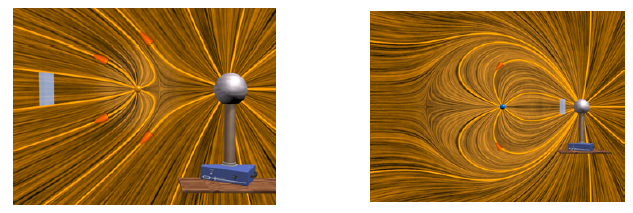
\includegraphics[width=0.8\textwidth]{figs/41a.png}
        \end{center}
        静电荷(Q)激发电场$\vec{E}$,静电荷通过电场发生相互作用. 
\end{frame}

\begin{frame}
    \frametitle{}    
    电场强度: \[\vec{E}=\frac{\vec{F}}{q}=\frac{1}{4\pi \epsilon_0}\frac{Q}{r^2}\vec{e}_r\]
    高斯定理(电通量):\[ \oint_S \vec{E}\cdot d \vec{S} = \frac{1}{\epsilon_0}\int_V \rho  d V \]  
    电势: \[ \varphi =\int^\infty_r \vec{E}\cdot d \vec{l} = \frac{1}{4\pi \epsilon_0}\frac{Q}{r}\]
    环路定理: \[ \oint_C \vec{E}\cdot d \vec{l} = 0\]
    两者关系: \[ \vec{E}=-\frac{\partial \varphi}{\partial n} \vec{e}_n=-\mathrm{Grad.} \varphi =-\nabla \varphi\]
    特点: 有源无旋
\end{frame}

\subsection{稳恒电流的磁场}

\begin{frame}
      \frametitle{电流相互作用}
        \begin{center}
             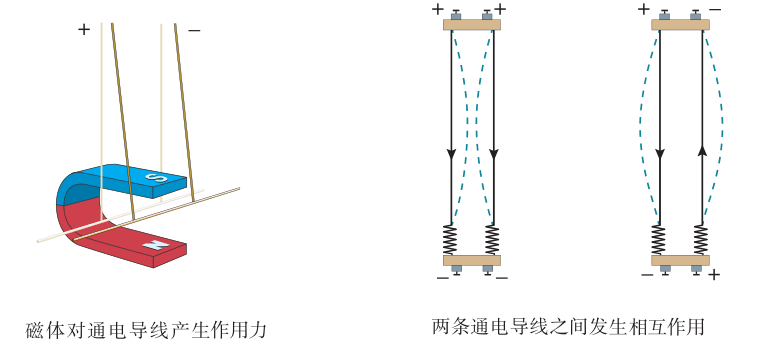
\includegraphics[width=0.8\textwidth]{figs/2022-04-04-11-09-40.png}
        \end{center}
        运动电荷(电流)激发电场和磁场$\vec{E}$,通过电磁场发生相互作用.  
\end{frame}

\begin{frame}
    \frametitle{}    
    磁感强度: \[d\vec{B}=\frac{\mu_0}{4\pi}\frac{\vec{I}d \vec{l}\times \vec{e}_r}{r^2}\]
    高斯定理(磁通量):\[ \oint_S \vec{B}\cdot d \vec{S} = 0 \] 
    环路定理: \[ \oint_C \vec{B}\cdot d \vec{l} = \mu_0 \int_s \vec{j}\times d \vec{S} \]
    磁矢势: \[\vec{A}=\frac{\mu_0}{4\pi} \int \frac{\vec{j}dV}  {r}\]
    特点: 有旋无源
\end{frame}

\subsection{交变电磁场}

\begin{frame}
    \frametitle{感应电场}
    电荷在电磁场中受力: \[ \vec{F}=q(\vec{E}+\vec{E_k}) = q(\vec{E}+\vec{v}\times \vec{B}) \]
    磁场变化产生感应电场:
    高斯定理:\[ \oint \vec{E_k}\cdot d \vec{S} = 0 \] 
    环路定理: \[ \oint \vec{E_k}\cdot d \vec{l} = - \int \frac{\partial \vec{B} }{\partial t} \times d \vec{S}\]
\end{frame}

\begin{frame}
    总电场(真空中): \[\vec{E}=\vec{E_k}+\vec{E_s} \] 
    总电场基本方程 \\ 
    高斯定理:\[ \oint \vec{E_k}\cdot d \vec{S} = \frac{1}{\epsilon_0}\int_V \rho  d V \]  
    环路定理: \[ \oint \vec{E_k}\cdot d \vec{l} = - \int \frac{\partial \vec{B} }{\partial t} \times d \vec{S}\]
\end{frame}

\begin{frame}
    \frametitle{位移电流}
    总电流密度: \[\vec{j}=\vec{j_D}+\vec{j_c}, \qquad  \vec{j_D}=\epsilon_0 \frac{\partial \vec{E}}{\partial t} \] 
    总磁场基本方程 \\
    高斯定理:\[ \oint_S \vec{B}\cdot d \vec{S} = 0 \] 
    环路定理: \[ \oint_C \vec{B}\cdot d \vec{l} = \mu_0 \int_s \vec{j}\times d \vec{S}+ \mu_0 \epsilon_0 \int \frac{\partial \vec{E}}{\partial t} \times \vec{S} \]
\end{frame}

\begin{frame}
    \frametitle{麦克斯韦方程}
    积分形式:
  \begin{center}
       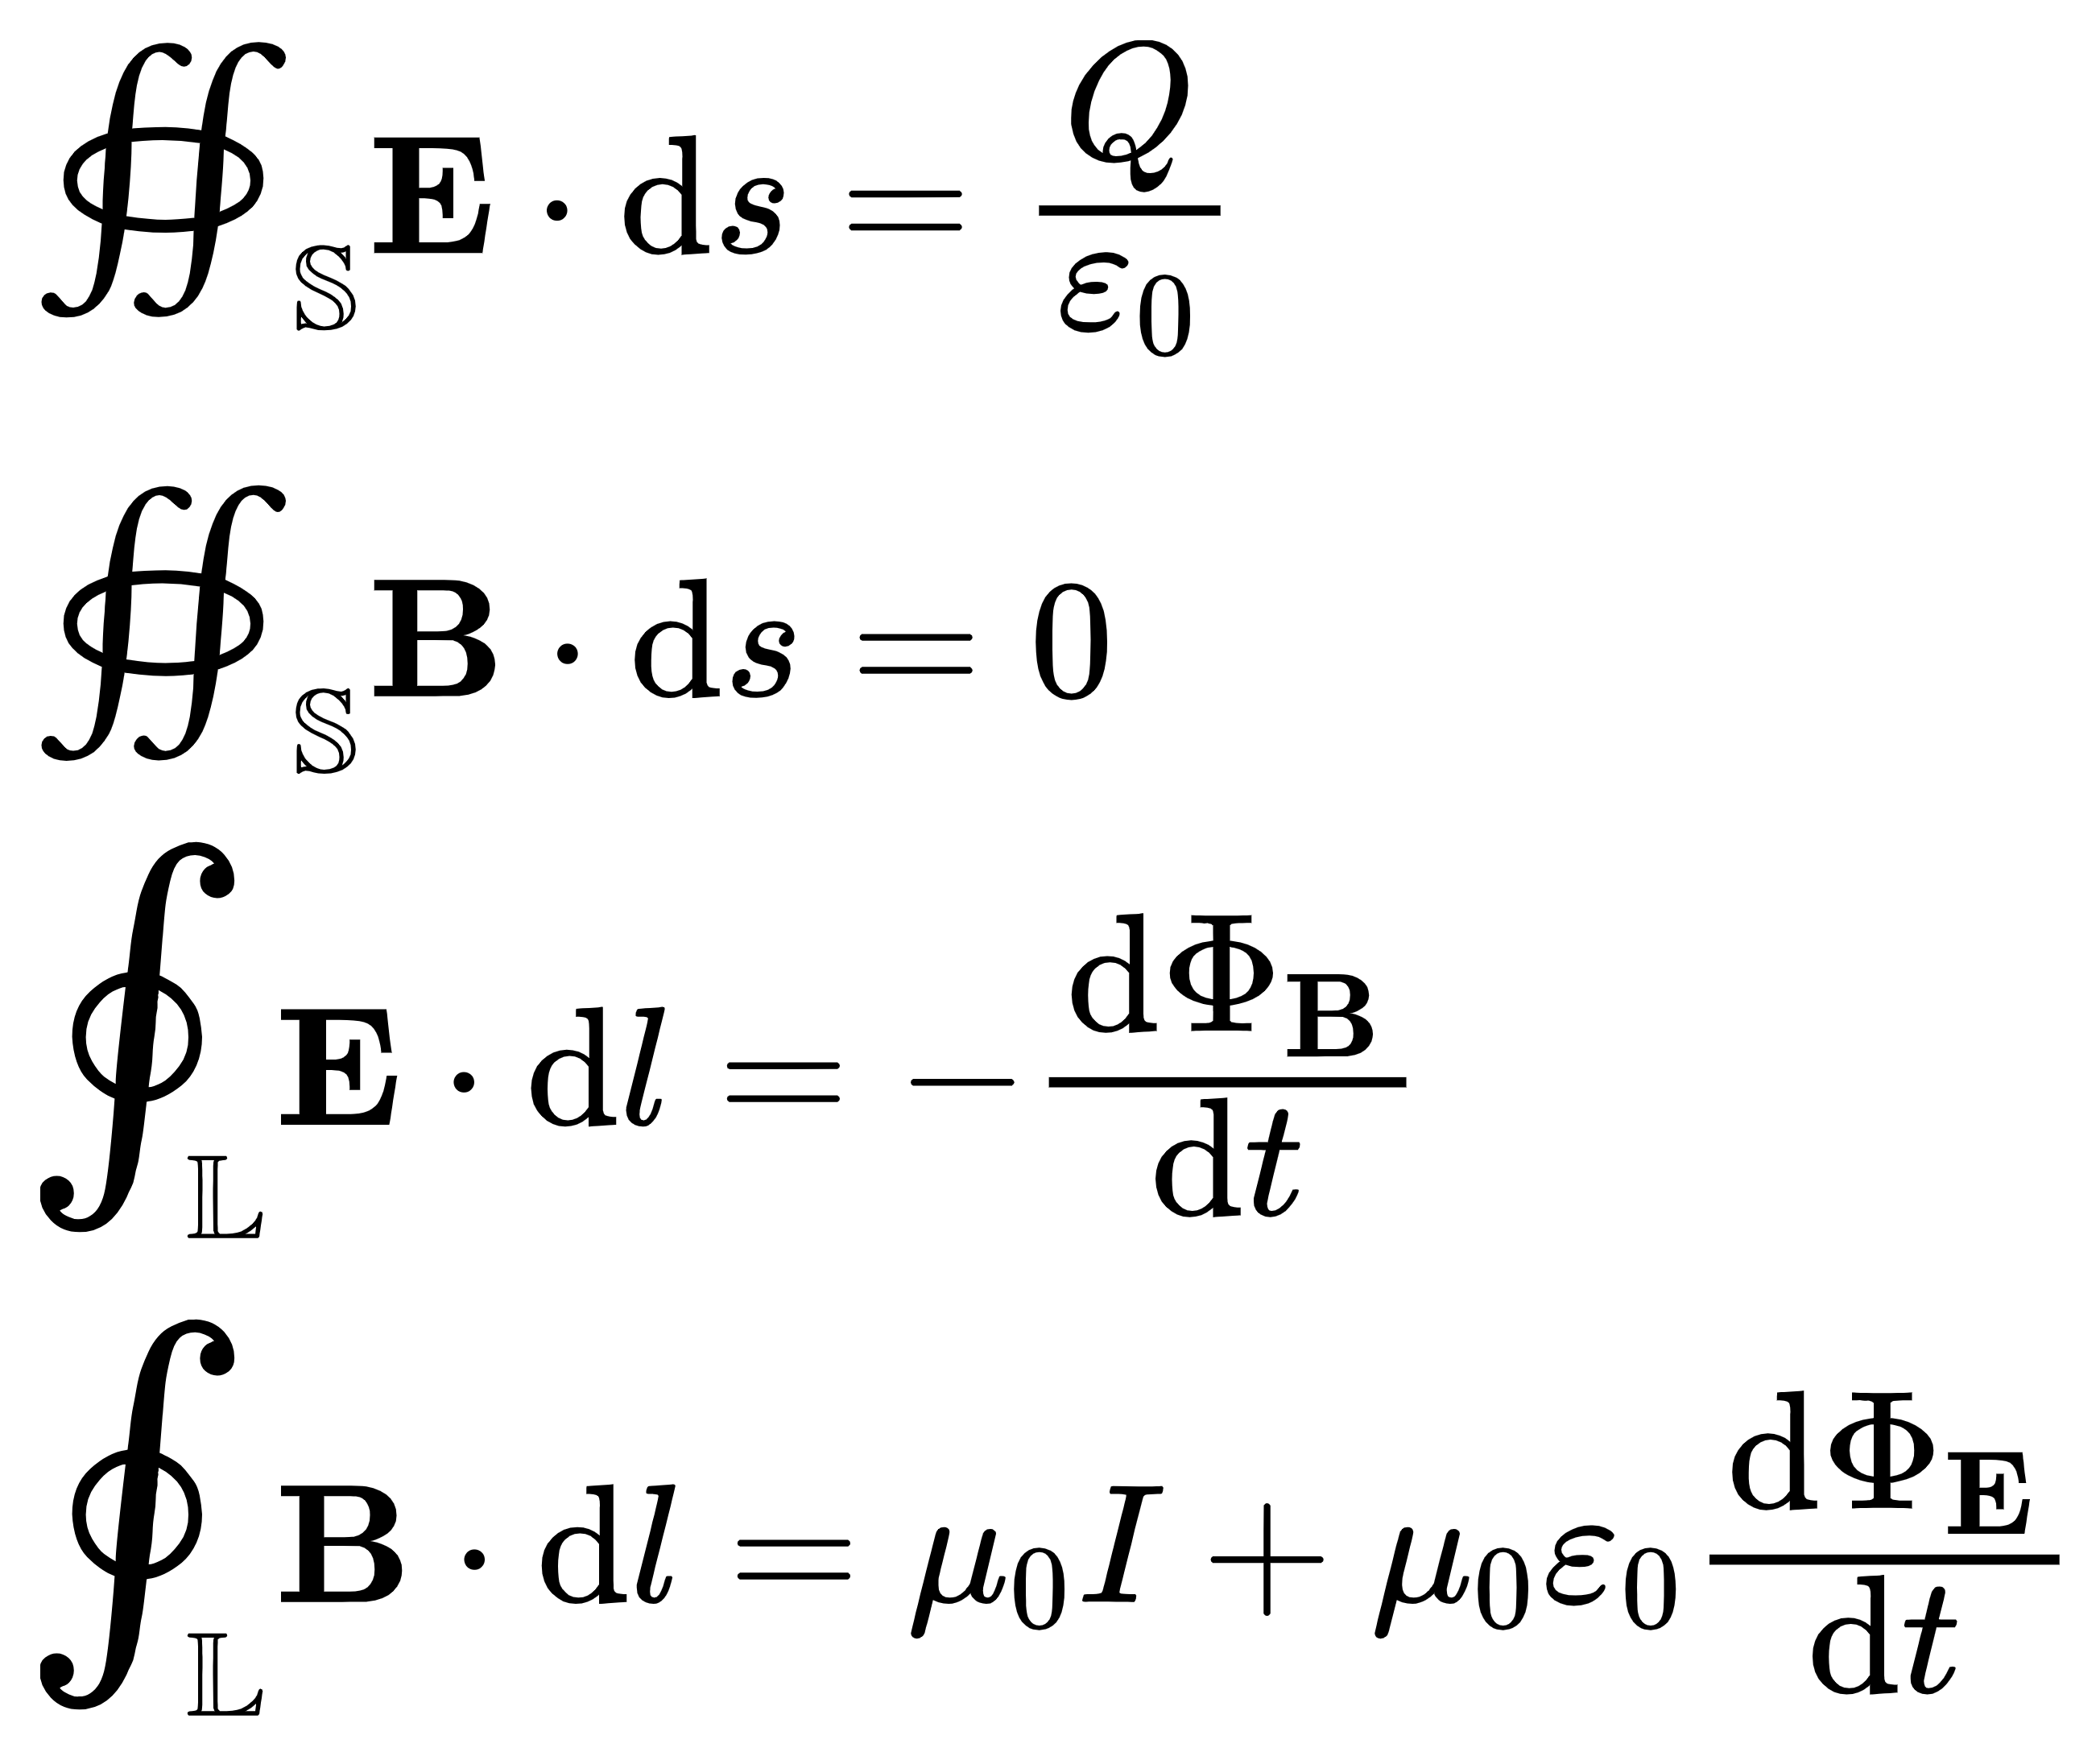
\includegraphics[width=0.4\textwidth]{figs/42.png}
  \end{center}
\end{frame}

\begin{frame}
      \frametitle{}
      微分形式:
      \[ \begin{array}{l}  
        \nabla \cdot \mathbf{E} =\cfrac{\rho}{\varepsilon _0}  \\  
        \nabla \cdot \mathbf{B} = 0 \\  
        \nabla \times  \mathbf{E} = -\cfrac{\partial \mathbf{B}}{\partial t }  \\  
        \nabla \times  \mathbf{B} = \mu _0\mathbf{J} + \mu _0\varepsilon_0 \cfrac{\partial \mathbf{E}}{\partial t }   
      \end{array} \] 
\end{frame}

\begin{frame}
      \frametitle{}
      介质中, 定义 电位移矢量$D$ 和 磁场强度 $H$
      \[ \vec{D}=\epsilon_0 \vec{E} + \vec{P} = \epsilon_0 \epsilon_r \vec{E},  \qquad \vec{H}=\frac{1}{\mu_0} \vec{B} -\vec{M}= \frac{1}{\mu_0\mu_r} \]
      麦克斯韦方程:
      \[ \begin{array}{l}  
        \nabla \cdot \mathbf{D} =\rho _f \\  
        \nabla \cdot \mathbf{B} = 0 \\  
        \nabla \times  \mathbf{E} = -\cfrac{\partial \mathbf{B}}{\partial t }  \\  
        \nabla \times  \mathbf{H} = \mathbf{J}_f +  \cfrac{\partial \mathbf{D}}{\partial t }   
      \end{array} \]
\end{frame}

\begin{frame}
    \frametitle{电磁场的能量}
      \begin{center}
           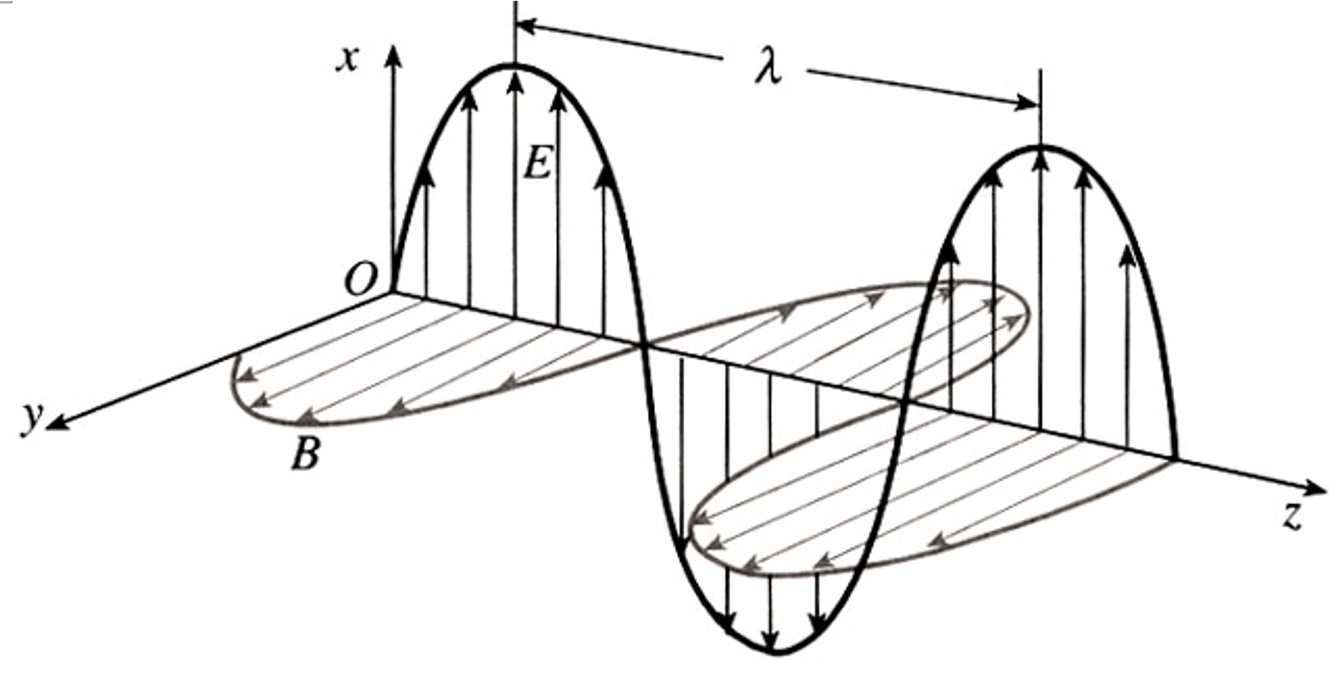
\includegraphics[width=0.55\textwidth]{figs/43.png}
      \end{center}
      能量密度: 
      \[ \omega = \frac{1}{2} (\epsilon_0 E^2 _x + \mu_0 H^2 _y) \]
      哈密顿量: \[ H = \frac{1}{2} \int_V (\epsilon_0 E^2 _x + \mu_0 H^2 _y) dV \]
\end{frame}

\subsection*{电磁波求解}

\begin{frame}
      \frametitle{电磁波} 
       对于真空 ($\rho _f =0, \mathbf{J}_f =0 $), 把 \[ \mathbf{B} = \mu_0 \mathbf{H}, \qquad  \mathbf{D} = \epsilon_0 \epsilon_r \mathbf{E} \]
      代入如下麦克斯韦方程
       \[ \nabla \times  \mathbf{H} = \mathbf{J}_f +  \cfrac{\partial \mathbf{D}}{\partial t } \]
      得: \[ \nabla \times \mathbf{B} = \mu_0\epsilon_0 \epsilon_r \cfrac{\partial \mathbf{E}} {\partial t } \]
    \[
    \begin{aligned}
        \nabla \times (\nabla \times  \mathbf{E}) &= - \nabla \times \cfrac{\partial \mathbf{B}}{\partial t } \\
        &= - \mu_0\epsilon_0 \epsilon_r \cfrac{\partial ^2 \mathbf{E}} {\partial t^2 }
    \end{aligned} \]
\end{frame}

\begin{frame}{}
由于
  \[
  \begin{aligned}
      \nabla \times (\nabla \times  \mathbf{E}) &=  \nabla (\nabla \cdot  \mathbf{E})- \nabla^2 \mathbf{E} \\
      &= - \nabla^2 \mathbf{E} 
  \end{aligned} \]
  得:
  \[
  \nabla^2 \mathbf{E}= \mu_0\epsilon_0 \epsilon_r \cfrac{\partial ^2 \mathbf{E}} {\partial t^2 }\]
  改写成
  \[\boxed{E_{tt} =c^2\nabla^2 \mathbf{E}}\]
  ~~\\
  这是波动方程的标准型(见数理方程)
\end{frame}

\begin{frame}
      \frametitle{}
      由于电磁波是横波, 当它在$z$方向转波时, 有$E_y=E_z=0, B_x=B_z=0$,考虑一个光学腔$0\leq z\leq L$\\ \vspace*{0.6em}
      令 $E_x =U(z)T(t)$ 分离变量,得解:
      \begin{enumerate}
		\IItem 固有值:$\displaystyle  \lambda_n=\frac{n^2\pi^2}{L^2}= k^2 _n $ 
		\IItem 固有解:$\displaystyle  U_n(z)=\sin (k_n z) $
        \IItem 基本解:$\displaystyle E_{x,n}(z,t) = T_n(t) U_n(z)=a_n \sin (k_j ct )\sin (k_n z) = a_n \sin (\nu_j t) \sin (k_n z) $
        \IItem 叠加解:$\displaystyle E_{x}(z,t) = \sum\limits_{n=1}^{\infty } a_n\sin (\nu_n t) \sin (k_n z) = \sum\limits_{n=1}^{\infty } a_n q (t) \sin (k_n z)$
	\end{enumerate}	      
\end{frame}

\begin{frame}
      \frametitle{}
      把解代入下式
      \[ \nabla \times \mathbf{B} = \mu_0\epsilon_0 \epsilon_r \cfrac{\partial \mathbf{E}} {\partial t } \]
      得: 
      \begin{enumerate}
        \IItem 叠加解:$\displaystyle H_{y}(z,t) = \sum\limits_{n=1}^{\infty } a_n \frac{\epsilon_0}{k_n}q' (t) \cos (k_n z)$
        \IItem 固有解正交归一化 $ \int^L _0 U_n(z) U_m(z)dz =\delta_{nm} $  \\ 
         得系数  $a_n $
	\end{enumerate}	
    结论: 电磁场的运动可分解为一系列基本模式的振动,在自由场条件下,振动是自由的,若有电荷或电流,变成受迫振动.
\end{frame}

\section{2. 电磁场的量子化}
\subsection{简振模展开}
\begin{frame}
    \frametitle{场与粒子}
    \begin{enumerate}
        \item 场是物质存在的基本形式
        \item 所有的粒子都是场的量子,分为费米子和玻色子两大类
        \item 场的量子与量子力学中的粒子并不完全一样,在非相对论近似下两都可以拟合在一起
        \item 光子无非相对论近似,不可能被看做量子力学中的粒子
        \item 电磁场量子化有着不同于一般意义的效应.
    \end{enumerate}
    物理问题:如何将电磁场中以场形式的能量,用腔中的模式来表达,变成一份一份的能量子(光子)。\\ 
    谐振子哈密顿量: $ H = \frac{p^2}{2m} +\frac{1}{2} \omega ^2 x^2 $
\end{frame}

\begin{frame}
  \frametitle{量子化标准化程序}
  \begin{enumerate}
    \item 写出经典哈密顿,改写为共轭变量形式, 并给出正则方程 
    \[ \begin{aligned}
      \frac{\mathrm{d}p_l}{\mathrm{d}t} &= - \frac{\partial H_l}{\partial q_l}  \\ 
      \frac{\mathrm{d}q_l}{\mathrm{d}t} &= \frac{\partial H_l}{\partial p_l} 
    \end{aligned} 
    \] 
    \item 共轭变量的算符满足量子力学基本对易关系
     \[ [q_l,p_m] =i\hbar \delta_{lm}\]
    \item 把哈密顿代入薛定谔方程,得量子解. 
    \[i\hbar \frac{\partial }{\partial t} \rs{ \Psi}  =H \rs{ \Psi}   \]
  \end{enumerate}
\end{frame}

\begin{frame}
  \frametitle{简振模展开}   
    注意电磁波的叠加解:
    \begin{enumerate}
        \IItem $\displaystyle E_{x}(z,t) = \sum\limits_{n=1}^{\infty } a_n q (t) \sin (k_n z)$
        \IItem $\displaystyle H_{y}(z,t) = \sum\limits_{n=1}^{\infty } a_n \frac{\epsilon_0}{k_n}q' (t) \cos (k_n z)$   
	\end{enumerate}	  
    电磁场按腔模式展开时, 电场的展开系数与各模的广义位置相关,磁场的展开系数与各模的广义动量相关.  写成三维形式,可以表示为:
    \[ \begin{aligned}
        \mathbf{E}( \mathbf{r},t) =& - \frac{1}{\sqrt{ \epsilon_0}} \sum_l ^\infty p_l(t) \mathbf{E}_l( \mathbf{r}) \\
        \mathbf{H}( \mathbf{r},t) =& - \frac{1}{\sqrt{ \mu_0}} \sum_l ^\infty \omega_l q_l(t) \mathbf{H}_l( \mathbf{r}) \\
     \end{aligned} 
    \]
    展开系数是$\mathbf{E}$和$\mathbf{H}$ 的矩阵表示.
\end{frame}

\begin{frame} 
    代回麦克斯韦方程, 得  
    \[ \begin{aligned}
        \ddot{p}_l &+ \omega_l ^2 p_l=0  \\ 
        \dot{q}_l &=p_l
     \end{aligned} 
    \] 
    因此, 电磁场的能量,可写成
    \[ \begin{aligned}
        H &= \frac{1}{2} \int_V (\mu_0 \mathbf{H}^2 + \epsilon_0 \mathbf{E}^2) dV \\ 
        &= \sum_l ^\infty \frac{1}{2}(p_l ^2 + \omega_l ^2 q_l ^2 ) \\ 
        &= \sum_l ^\infty H_l  
     \end{aligned} 
    \] 
    谐振子: $ H = \frac{p^2}{2m} +\frac{1}{2} \omega ^2 x^2 $, 电磁场可视为一组无耦合离散谐振子的无穷集.
\end{frame}

\begin{frame}
    \frametitle{求解}
          对哈密顿$H_l= \frac{1}{2}(p_l ^2 + \omega_l ^2 q_l ^2 )$求导,得哈密顿运动方程
        \[ \begin{aligned}
            \frac{\mathrm{d}p_l}{\mathrm{d}t} &= - \frac{\partial H_l}{\partial q_l} = - \omega ^2 _l q_l \\ 
            \frac{\mathrm{d}q_l}{\mathrm{d}t} &= \frac{\partial H_l}{\partial p_l} =p_l
         \end{aligned} 
        \] 
    说明 $ p_l $ 和$q_l$ 是 电磁场的一对正则共轭变量.  令  
    \[ \begin{aligned}
        a_l &= \frac{1}{\sqrt{2\hbar \omega_l}} (\omega_lq_l+i p_l) \\ 
        a_l ^* &= \frac{1}{\sqrt{2\hbar \omega_l}} (\omega_lq_l-i p_l)  
     \end{aligned} 
    \] 
    哈密顿变为
    \[ H_l= \frac{1}{2}\hbar \omega_l (a_l a_l ^* + a_l ^*a_l )  \]
\end{frame}


\begin{frame}
    \frametitle{}
     反向求得 
     \[ \begin{aligned}
        q_l &= \sqrt{\frac{\hbar}{ 2\omega_l}} (a_l+ a_l ^*) \\ 
        p_l ^* &= -\sqrt{\frac{\hbar\omega_l}{2 }} (a_l- a_l ^*)  
     \end{aligned} 
    \] 
     代回哈密顿运动方程: 
     \[ \begin{aligned}
        \frac{\mathrm{d}a_l}{\mathrm{d}t} &= - i\omega_l a_l \\ 
        \frac{\mathrm{d}a_l ^*}{\mathrm{d}t} &=  i \omega_l a_l ^*
     \end{aligned} 
    \] 
    解得 
    \[ \begin{cases}
       a_l(t) &= a_l(0)e^{- i\omega_l t} \\ 
       a_l ^*(t) &= a_l ^* (0) e^{i \omega_l t}
    \end{cases} 
   \] 
   说明腔场为驻波解!
\end{frame}


\subsection{行波展开}

\begin{frame}
    \frametitle{自由空间电磁场}
    自由空间电磁场模为平面波(行波), 解的形式为:
    \[  \hat{e}_\sigma exp (\pm i (\omega_k t - \mathbf{k}\cdot \mathbf{r})), \qquad k^2 =\frac{\omega_k ^2}{c^2} \]
    式中 $\hat{e}_\sigma $ 为偏振方向上的单位矢量, $\sigma=1 ~\text{or} ~2$代表两个振动方向, 它们相互正交且都与波矢$\mathbf{k}$正交. \\ \vspace*{1em} 
    经箱归一化, 可离散化行波, 得 
    \[ \mathbf{k} = \frac{2\pi}{L} (l_1 \mathbf{i} + l_2 \mathbf{j}+ l_3 \mathbf{k}), \qquad l_i= 0, \pm 1, \pm 2, \cdots \]
    行波本征模为
    \[ \mathbf{u}_{k\sigma} (\mathbf{r}) = \hat{e}_\sigma e^{i \mathbf{k}\cdot \mathbf{r}}\]
\end{frame}

\begin{frame}
  \frametitle{行波展开}
  自由空间电磁场按行波展开
  \[   \begin{aligned}
    \mathbf{E} (\mathbf{r},t) &=i \sum^\infty _{k,\sigma} (\frac{\hbar\omega_k}{2 \epsilon_0 V } )^{1/2} \hat{e}_\sigma [ a_{k\sigma} (t) e^{i \mathbf{k}\cdot \mathbf{r}} - a ^* _{k\sigma} (t)  e^{-i \mathbf{k}\cdot \mathbf{r}}] \\
  \mathbf{H} (\mathbf{r},t) &=i \sum^\infty _{k,\sigma} (\frac{\hbar\omega_k}{2 \mu_0 V } )^{1/2} (\hat{e}_k \times \hat{e}_\sigma) [ a_{k\sigma} (t) e^{i \mathbf{k}\cdot \mathbf{r}} - a ^* _{k\sigma} (t)  e^{-i \mathbf{k}\cdot \mathbf{r}}] 
\end{aligned} 
  \]
  箱内总能量:
  \[ \begin{aligned}
    H &= \frac{1}{2} \int_V (\mu_0 \mathbf{H}^2 + \epsilon_0 \mathbf{E}^2) dV \\ 
    &= \frac{1}{2}\sum^\infty _{k,\sigma} \hbar \omega_k (a_{k\sigma} a_{k\sigma} ^* + a_{k\sigma} ^*a_{k\sigma} )   \\ 
    &= \frac{1}{2}\sum^\infty _{k,\sigma} (p_{k\sigma} ^2 + \omega_k ^2 q_{k\sigma} ^2 )  = \sum^\infty _{k,\sigma} H_{k\sigma}
 \end{aligned} 
\] 
\end{frame}

\begin{frame}
    \frametitle{}
    哈密顿运动方程
    \[ \begin{aligned}
        \frac{\mathrm{d}p_{k\sigma}}{\mathrm{d}t} &= - \frac{\partial H_{k\sigma}}{\partial q_{k\sigma}} = - \omega ^2 _{k\sigma} q_{k\sigma} \\ 
        \frac{\mathrm{d}q_{k\sigma}}{\mathrm{d}t} &= \frac{\partial H_{k\sigma}}{\partial p_{k\sigma}} =p_{k\sigma}
     \end{aligned} 
    \] 
    小结: 能过光腔解和行波解, 可以得到电磁场的谐振模(驻波)或行波模(平面波)的线性叠加解. 下面对单模进行量子化.
\end{frame}

\subsection{单模量子化}

\begin{frame}
  \frametitle{产生湮灭算符}
(1) 由正则共轭变量写出产生湮灭算符
 \[\begin{aligned}
  a &= \frac{1}{\sqrt{2\hbar \omega}} (\omega q+i p) \\ 
  a ^\dagger &= \frac{1}{\sqrt{2\hbar \omega}} (\omega q - i p)
  \end{aligned}\]
\end{frame}


\begin{frame} 
(2) 基于正则共轭变量量子化条件,
  \[[ q,  p]= i \hbar\]
  求产生湮灭算符对易关系 \\
  {\解} ~ 
  \[\begin{aligned}
    [a,a ^\dagger] &= a a ^\dagger- a ^\dagger a \\ 
    &= (\frac{1}{\sqrt{2\hbar \omega}})^2 [(\omega q+i p)(\omega q - i p)-(\omega q-i p)(\omega q + i p)] \\ 
    &= (\frac{1}{\sqrt{2\hbar \omega}})^2  2i\omega( p q - q  p) \\ 
    &= - (\frac{1}{\sqrt{2\hbar \omega}})^2  2i\omega[ q,  p]  \\
    &= - (\frac{1}{\sqrt{2\hbar \omega}})^2  2i\omega (i\hbar)  \\
    &= 1
  \end{aligned}\]
\end{frame}

\begin{frame} 
  (3) 单模驻波场相关力学量算符 \\ 
  产生湮灭算符
  \[\begin{aligned}
    a &= \frac{1}{\sqrt{2\hbar \omega}} (\omega q+i p) \\ 
    a ^\dagger &= \frac{1}{\sqrt{2\hbar \omega}} (\omega q - i p)
    \end{aligned}\]
   反向求得正则共轭变量算符
  \[ \begin{aligned}
    q &= \sqrt{\frac{\hbar}{2 \omega}} (a + a ^\dagger ) \\ 
    p &= i\sqrt{\frac{\hbar\omega}{2 }} (a^\dagger -a)  
  \end{aligned} 
  \] 
\end{frame}

\begin{frame}
  代入,得哈密顿算符
  \[ \begin{aligned}
    H_l&= \frac{1}{2}(p_l ^2 + \omega_l ^2 q_l ^2 ) \\ 
    H& = \frac{1}{2} [ (i\sqrt{\frac{\hbar\omega}{2 }} (a^\dagger -a) )^2 + \omega ^2  (\sqrt{\frac{\hbar}{2 \omega}} (a + a ^\dagger ))^2] \\
    & = \frac{1}{2} [ (i\sqrt{\frac{\hbar\omega}{2 }} (a^\dagger -a) )^2 +  (\sqrt{\frac{\hbar\omega}{2 }} (a + a ^\dagger ))^2] \\
    & = \frac{1}{4}\hbar \omega [(a + a ^\dagger )^2-( a ^\dagger - a)^2 ] \\
    & = \frac{1}{4}\hbar \omega [2a a ^\dagger -  2a^\dagger a  + 4a ^\dagger a  ] \\
    &=  \hbar \omega a ^\dagger a + \frac{1}{2}\hbar \omega 
  \end{aligned} 
  \] 
\end{frame}

\begin{frame} 
  代入得电磁场强度算符,
  \[ \begin{aligned}
    \mathbf{E}_l( \mathbf{r})& = - \frac{1}{\sqrt{ \epsilon_0}} p_l \mathbf{E}_l( \mathbf{r}) \\
    \mathbf{E}&= - \frac{1}{\sqrt{ \epsilon_0}} (i\sqrt{\frac{\hbar\omega}{2 }} (a^\dagger -a)) \mathbf{E}( \mathbf{r}) \\
    &= i \sqrt{\frac{\hbar\omega}{2 \epsilon_0}} \mathbf{E}( \mathbf{r}) (a - a^\dagger) \\ 
    \mathbf{H}_l( \mathbf{r}) &=- \frac{1}{\sqrt{ \mu_0}}  \omega_l q_l \mathbf{H}_l( \mathbf{r}) \\
    \mathbf{H} &= \frac{1}{\sqrt{ \mu_0}}  \omega \sqrt{\frac{\hbar}{2 \omega}} (a + a ^\dagger ) \mathbf{H}( \mathbf{r}) \\
    &= \sqrt{\frac{\hbar\omega}{2 \mu_0}} \mathbf{H}( \mathbf{r}) (a + a^\dagger)
 \end{aligned} 
\]
\end{frame}

\begin{frame}
  \frametitle{产生湮灭算符的性质}
  $ a \not =  a^\dagger $, 不是自伴算符,不具厄密性. 有必要研究其具体性质.\\ 
对于能量第n个本征态,  
  \[ H  \rs{n} = E_n  \rs{n}, \quad  aH  \rs{n} =E_n a \rs{n}\]
  \[
  \begin{aligned}
        H a \rs{n} &= ( \hbar \omega a ^\dagger a + \frac{1}{2}\hbar \omega )a \rs{n} \\ 
        &=  ( \hbar \omega  a ^\dagger a a  + \frac{1}{2}\hbar \omega a ) \rs{n} \\ 
        &=  ( \hbar \omega  (-1+a a ^\dagger )a + \frac{1}{2}\hbar \omega a ) \rs{n} \\ 
        &=  ( \hbar \omega  a a ^\dagger a -  a \frac{1}{2}\hbar \omega ) \rs{n} \\ 
        &=  a( \hbar \omega   a ^\dagger a -  \frac{1}{2}\hbar \omega ) \rs{n} 
  \end{aligned}
  \]
\end{frame}

\begin{frame}
  \frametitle{}
  \[ 
  \begin{aligned}
    H a \rs{n}  &=  a( \hbar \omega   a ^\dagger a +  \frac{1}{2}\hbar \omega  - \hbar \omega ) \rs{n} \\ 
        &=  (aH - a \hbar \omega ) \rs{n} \\ 
        &=  (E_n -  \hbar \omega ) a\rs{n} \\ 
  \end{aligned}
  \]
  也就是说 $a \rs{n} $ 也是能量本性态, 本征值为 $E_n -  \hbar \omega = E_{n-1} $ 即有一份能量$ \hbar \omega $ 被湮灭, 故称 $a$ 为 湮灭算符\\ 
  性质1: 
  \[ \boxed{a \rs{n}= D_n\rs{n-1}} \]
  ~~\\ 
  \[ H a \rs{n} =   H  \rs{n-1} = E_{n-1} \rs{n-1} = (E_{n}-\hbar \omega) \rs{n-1}\]
\end{frame}

\begin{frame}
同理可证: 
\[  H a^\dagger \rs{n}  =  (E_n +  \hbar \omega ) a^\dagger \rs{n} \]
也就是说 $a^\dagger\rs{n} $ 也是能量本性态, 本征值为 $E_n + \hbar \omega = E_{n-1} $ 即产生一份能量$ \hbar \omega $, 故称 $a^\dagger$ 为产生算符\\ 
性质2: 
\[ \boxed{a^\dagger \rs{n}= C_n \rs{n+1}} \]

\end{frame}

\begin{frame}
    \frametitle{真空态}
    本征能量可无限地增加,但不能被无限湮灭,设最小的为$E_0$, 对应本征态$\rs{0}$\\ 
    性质3:
    \[ \boxed{a \rs{0}= 0 }\]
    ~~\\ 
    $H=\hbar \omega a ^\dagger a + \frac{1}{2}\hbar \omega, \qquad H-\frac{1}{2}\hbar \omega=\hbar \omega a ^\dagger a $ 
    \[ 
  \begin{aligned}
    (H-\frac{1}{2}\hbar \omega) \rs{0} &= \hbar \omega a ^\dagger a \rs{0} = \hbar \omega a ^\dagger 0 = 0 \\ 
    H \rs{0} &= \frac{1}{2}\hbar \omega \rs{0}=E_0 \rs{0} 
  \end{aligned}
  \] 
  性质4:  \[ \boxed{E_0=\dfrac{1}{2}\hbar \omega} \]
\end{frame}

\begin{frame}
    \frametitle{能量本征值}
     从真空态出发, 相继使用产生算符,每次产生一份能量 $ \hbar \omega$, 因此能量本征值为
     \[E_n = (n+\frac{1}{2})\hbar \omega, \qquad n=0,1,2, \cdots  \] 
  ~~\\
    粒子数态:\\
     对电磁场来说, 单模场的本征态$\rs{n}$描述的是该模上有$n$个光子, 每个光子的能时都是 $\hbar \omega$ 即 :$\rs{n}$态描述的是含有$n$个光量子的态. 因此,能量本征态$\rs{n}$也称为粒子数态. 占有数算符为$ N=a^\dagger a $, 有本征方程:
    \[ a^\dagger a \rs{n}= n\rs{n}\] 
\end{frame}

\begin{frame}
  \frametitle{归一化系数}
  产生湮灭算符分别产生和消灭这个模式的一个光子
  \[ {a \rs{n}= D_n\rs{n-1}}, \qquad a^\dagger \rs{n}= C_n \rs{n+1} \]  
  \[ 
    \begin{aligned}
      a^\dagger a \rs{n} &= a^\dagger D_n\rs{n-1} \\ 
      &= D_n C_{n-1} \rs{n} = n \rs{n} \\ 
      D_n C_{n-1}&=n \qquad \cdots (1)
    \end{aligned}
    \] 
    \[ 
      \begin{aligned}
        D_n &=  \lcr{n-1}{a}{n} \\
        &=  (\lcr{n}{a^\dagger }{n-1})^* \\
        &= C_{n-1} ^*   \qquad \cdots (2)
      \end{aligned}
      \] 
      联立(1)(2), 得 $C_{n-1}=\sqrt{n}= D_n, C_{n}=\sqrt{n+1} $
\end{frame}

\begin{frame}
    \frametitle{Fock表象}
    占有数算符$N=a^\dagger a $的本征函数系是正交归一完备系, 构成的表象称为粒子数表象,也称为Fock表象. \\
    \例[1.试证明$Fock$ 态下电磁场的电场强度平均值为零]{}
    \证~设电磁场处于$Fock$ 态 $\rs{n}$
    \[ 
      \begin{aligned}
        \lcr{n}{\mathbf{E}}{n} &= \lcr{n}{\i \sqrt{\frac{\hbar\omega}{2 \epsilon_0}} \mathbf{E}( \mathbf{r}) (a - a^\dagger) }{n}   \\ 
        &= \lcr{n}{\i \sqrt{\frac{\hbar\omega}{2 \epsilon_0}} \mathbf{E}( \mathbf{r})a }{n} - \lcr{n}{\i \sqrt{\frac{\hbar\omega}{2 \epsilon_0}} \mathbf{E}( \mathbf{r})a^\dagger }{n}  \\ 
        &= 0-0 =0 
      \end{aligned}
      \]   
      * 相位随机性导致测量平均值为零! Fock表象一般用于处理小粒子数的情况. 
\end{frame}

\begin{frame}
    \frametitle{单模场的量子涨落}
    \例[2.考虑一维单模驻波场, 求电场和磁场强度的量子涨落]{}
    \解~一维单模驻波场的电场和磁场算符为  
    \[ \begin{aligned}
      E_x(z,t)
      &= -i \sqrt{\frac{\hbar\omega}{\epsilon_0 L}} \sin kz (a^\dagger(t)-a(t) ) \\ 
      H_y(z,t)  
      &= \sqrt{\frac{\hbar\omega}{2 \mu_0 L}} \cos kz (a(t) + a^\dagger(t))
   \end{aligned} \]
   设光场处于FOCK态$\rs{n}$, 有:
   \[ \lcr{n}{E_x(z,t)}{n} = \lcr{n}{H_y(z,t)}{n} =0\]
\end{frame}

\begin{frame}
    \frametitle{}
    令 $E_0= \sqrt{\dfrac{\hbar\omega}{\epsilon_0 L}}$
    \[ \begin{aligned}
      \lcr{n}{E^2_x}{n} &= \lcr{n}{-E^2_0 \sin^2 kz (a^\dagger(t)-a(t))^2}{n} \\
      &= 2 E^2_0 \sin^2 kz \lcr{n}{a^\dagger a}{n} \\ 
      &= 2 E^2_0 \sin^2 kz \lcr{n}{n+\frac{1}{2}}{n} \\ 
      &= 2 (n+\frac{1}{2})E^2_0 \sin^2 kz  
   \end{aligned} \]
   量子涨落: 
   \[
  \begin{aligned}
         \langle \Delta E_x\rangle &= \sqrt{\langle (\Delta E_x)^2\rangle} = \langle (E^2_x)\rangle - \langle E_x\rangle ^2 \\
         &= \sqrt{2} \sqrt{n+\frac{1}{2}} E_0 \left|\sin kz \right| 
  \end{aligned} \]
  即使没有激发(n=0),依然存在真空涨落$ E_0 \left|\sin kz \right|  $  
\end{frame}

\section{3. 辐射场}
\subsection{密度算符}
\begin{frame}
    \frametitle{密度算符的定义}
      纯态: 用确定态矢量$\rs{\psi}$完全描述体系的状态, 基于外积,可以定义密度算符:
    \[ \rho =\rl{\psi}{\psi} \]
    则,算符A的平均值为
    \[ \overline{A} =\lcr{\psi}{A}{\psi} =tr(A\rho)\]
\end{frame}

\begin{frame}
    \frametitle{}
    混态: 不能用确定的态,而是用一组态矢量$\{ \rs{\psi_n}\}$才能完全描述体系的状态, 若用$P_n$ 表示用$\rs{\psi_n}$ 描述体系的概率, 也可定义密度(矩阵)算符
    \[ \rho =\sum_nP_n\rl{\psi_n}{\psi_n} \]
    则,算符A的平均值为
    \[ \overline{A} =\sum_n P_n\lcr{\psi_n}{A}{\psi_n} =tr(A\rho)\]
    \证~由矩阵的迹的定义式  
    \[\begin{aligned}
        tr(A\rho) &= \sum_i \lcr{i}{A\rho}{i} \\
        &= \sum_{i,n} \lcr{i}{AP_n}{\psi_n}\lr{\psi_n}{i} \\
        &= \sum_{i,n} \lr{\psi_n}{i} \lcr{i}{AP_n}{\psi_n}\\
        &= \sum_{n} P_n\lcr{\psi_n}{A}{\psi_n}
    \end{aligned}\]  
\end{frame}

\begin{frame}
    \frametitle{密度算符的性质}
    \textbf{性质1}.试证明密度算符是厄密算符 \\ 
    \证~
    \[ \begin{aligned}
      \lcr{\Psi}{\rho}{\varphi} &= \sum_n P_n\lcr{\Psi}{\rl{\psi_n}{\psi_n}}{\varphi} \\
      &= \sum_n P_n(\lcr{\varphi}{\rl{\psi_n}{\psi_n}}{\Psi})^* \\
      &= (\lcr{\varphi}{\rho}{\Psi})^* 
\end{aligned} \]    
\end{frame}

\begin{frame}
    \frametitle{}
    \textbf{性质2}.试证明$Tr \rho=1$ \\ 
    \证~
    \[ \begin{aligned}
      Tr \rho &= \sum_{jj} \rho_{jj} \\ 
      &= \sum_{n,j} P_n\rs{\psi_n} \rl{j}{j} \ls{\psi_n} \\
      &= \sum_{n,j} P_n \lr{j}{\psi_n} \lr{\psi_n}{j} \\
      &= \sum_{n,j} P_n \left|c_{nj}\right|^2 \\
      &= \sum_{n} P_n \sum_{j}\left|c_{nj}\right|^2 \\
      &=1
\end{aligned} \]   
\end{frame}

\begin{frame}
  \frametitle{}
  \textbf{性质3}.纯混态判据 \\ 
  \[ \begin{cases}
  \text{纯态}: Tr \rho^2=1 \\
  \text{混态}: Tr \rho^2<1 \\
  \end{cases} \]
  \证~TODO
  \[ \begin{aligned}
    Tr \rho &= \sum_{jj} \rho_{jj} \\ 
    &= \sum_{n,j} P_n\rs{\psi_n} \rl{j}{j} \ls{\psi_n} \\
    &= \sum_{n,j} P_n \lr{j}{\psi_n} \lr{\psi_n}{j} \\
    &= \sum_{n,j} P_n \left|c_{nj}\right|^2 \\
    &= \sum_{n} P_n \sum_{j}\left|c_{nj}\right|^2 \\
    &=1
\end{aligned} \]   
\end{frame}

\begin{frame}
  \frametitle{}
  \textbf{性质4}.密度算符的运动方程 \\ 
  \[ i\hbar \frac{\partial \rho}{\partial t} = [H,\rho]\]
  \证~
  \[ \begin{aligned}
    i\hbar \frac{\partial \rho}{\partial t}  &= i\hbar \frac{\partial }{\partial t} \sum_nP_n\rl{\psi_n}{\psi_n}  \\ 
    &= \sum_nP_n [i\hbar\frac{\partial \rs{\psi_n} }{\partial t} \ls{\psi_n} + \rs{\psi_n} i\hbar\frac{\partial \ls{\psi_n}}{\partial t} ] \\
    &= \sum_nP_n [ H \rs{\psi_n} \ls{\psi_n} - \rs{\psi_n} \ls{\psi_n}H ] \\
    &= [ H \rho  - \rho H ] \\
    &= [ H ,\rho] 
\end{aligned} \]   
\end{frame}

\subsection{辐射场}